\documentclass[11pt,a4paper]{report}

% Packages and commands file
\usepackage[utf8]{inputenc}
\usepackage[T1]{fontenc}
\usepackage[english]{babel}
\usepackage{amsmath}
\usepackage{ae}
\usepackage{icomma}
\usepackage{units}
\usepackage{color}
\usepackage{graphicx}
\usepackage{epstopdf}
\usepackage{subfigure}
\usepackage{bbm}
\usepackage{caption}
\usepackage{natbib}
\usepackage{multirow}
\usepackage{array}
\usepackage{geometry}
\usepackage{fancyhdr}
\usepackage{fncychap}
\usepackage[hyphens]{url}
\usepackage[breaklinks,pdfpagelabels=false]{hyperref}
\usepackage{lettrine}
\usepackage{eso-pic}

\newcommand{\rd}{\ensuremath{\mathrm{d}}}
\newcommand{\id}{\ensuremath{\,\rd}}
\newcommand{\degC}{\ensuremath{\,\unit{^\circ C}}}

% Fancyheader shortcuts
\newcommand{\setdefaulthdr}{%
\fancyhead[L]{\slshape \rightmark}%
\fancyhead[R]{\slshape \leftmark}%
\fancyfoot[C]{\thepage}%
}
\newcommand{\setspecialhdr}{%
\fancyhead[L]{ }%
\fancyhead[R]{\slshape \leftmark}%
\fancyfoot[C]{\thepage}%
}

\newcommand{\mail}[1]{\href{mailto:#1}{\nolinkurl{#1}}}
\newcommand{\backgroundpic}[3]{%
	\put(#1,#2){
		\parbox[b][\paperheight]{\paperwidth}{%
			\centering
			\includegraphics[width=\paperwidth,height=\paperheight,keepaspectratio]{#3}
			\vfill
}}}




\graphicspath{{./include/images/}}

% Settings (Metadata)
% References, choose bst-file
\bibliographystyle{plainnat}

% PDF Metadata and link styles
\hypersetup{
		pdftitle={Master's Thesis: },%
		pdfauthor={Erik Brännström},%
    colorlinks=true,%
    citecolor=black,%
    filecolor=black,%
    linkcolor=black,%
    urlcolor=black
}

% Dropping initial letter color
\renewcommand{\LettrineFontHook}{\color[gray]{0.5}}

% Chapter headings style (fncychap)
\makeatletter
\ChNumVar{} % sets the style for digit
\ChTitleVar{\Huge\bfseries\centering} % sets the style for title
\ChRuleWidth{4pt} % Set RW=4pt
\ChNameUpperCase % Make name uppercase
\renewcommand{\DOCH}{
\centering
{\CNoV {\fontsize{60pt}{20pt}\selectfont\thechapter} }
\vskip 40\p@}
\renewcommand{\DOTI}[1]{%
\CTV\FmTi{#1}\par\nobreak
\vskip 40\p@}
\renewcommand{\DOTIS}[1]{%
\CTV\FmTi{#1}\par\nobreak
\vskip 40\p@}
\makeatother

% Single page abstract
\renewenvironment{abstract}%
{\begin{center} \bfseries \abstractname \end{center}}%
{\vspace{2\baselineskip}}%

% Figure & Table captions
\captionsetup{margin=10pt,font=small,labelfont=bf}
\captionsetup[table]{position=top}
\setlength{\extrarowheight}{4pt}
\addtolength{\headheight}{\baselineskip}

% Fancyheader (see packagescommands.tex for default/special)
\pagestyle{fancy}
\setdefaulthdr

% Stolen settings (unknown origin):
% Alter some LaTeX defaults for better treatment of figures:
% See p.105 of "TeX Unbound" for suggested values.
% See pp. 199-200 of Lamport's "LaTeX" book for details.
%   General parameters, for ALL pages:
\renewcommand{\topfraction}{0.9}	% max fraction of floats at top
\renewcommand{\bottomfraction}{0.8}	% max fraction of floats at bottom
%   Parameters for TEXT pages (not float pages):
\setcounter{topnumber}{2}
\setcounter{bottomnumber}{2}
\setcounter{totalnumber}{4}     % 2 may work better
\setcounter{dbltopnumber}{2}    % for 2-column pages
\renewcommand{\dbltopfraction}{0.9}	% fit big float above 2-col. text
\renewcommand{\textfraction}{0.07}	% allow minimal text w. figs
%   Parameters for FLOAT pages (not text pages):
\renewcommand{\floatpagefraction}{0.7}	% require fuller float pages
% N.B.: floatpagefraction MUST be less than topfraction !!
\renewcommand{\dblfloatpagefraction}{0.7}	% require fuller float pages

% remember to use [htp] or [htpb] for placement

\begin{document}

% Title page and abstract
% Chalmers title page
\begin{titlepage}

\AddToShipoutPicture{\backgroundpic{-4}{56.7}{./include/images/frontpage}}
\mbox{}
\vfill
\addtolength{\voffset}{2cm}
\begin{flushleft}
	{\noindent {\Huge Automated analysis and planning of social network marketing} \\[0.5cm]
	\emph{\Large Master's Thesis in Software Engineering} \\[.8cm]

	{\huge ERIK BRÄNNSTRÖM}\\[.8cm]

	{\Large Division of Software Engineering \\
	\textsc{Chalmers University of Technology} \\
	Göteborg, Sweden 2012 \\
	Master's Thesis 2012:X\\
	}
	}
\end{flushleft}

\end{titlepage}
\ClearShipoutPicture
% End Chalmers title page

\pagestyle{empty}
\newpage
\clearpage
\mbox{}
\newpage
\clearpage
\thispagestyle{empty}

\onecolumn
\begin{abstract}
Lorem ipsum dolor sit amet, consectetur adipisicing elit, sed do eiusmod tempor incididunt ut labore et dolore magna aliqua. Ut enim ad minim veniam, quis nostrud exercitation ullamco laboris nisi ut aliquip ex ea commodo consequat. Duis aute irure dolor in reprehenderit in voluptate velit esse cillum dolore eu fugiat nulla pariatur. Excepteur sint occaecat cupidatat non proident, sunt in culpa qui officia deserunt mollit anim id est laborum.
\end{abstract}

\newpage
\clearpage
\mbox{}
\newpage
\clearpage
\thispagestyle{empty}
\section*{Acknowledgements}
Lorem ipsum dolor sit amet, consectetur adipisicing elit, sed do eiusmod tempor incididunt ut labore et dolore magna aliqua. Ut enim ad minim veniam, quis nostrud exercitation ullamco laboris nisi ut aliquip ex ea commodo consequat. Duis aute irure dolor in reprehenderit in voluptate velit esse cillum dolore eu fugiat nulla pariatur. Excepteur sint occaecat cupidatat non proident, sunt in culpa qui officia deserunt mollit anim id est laborum. \\[1cm]

\hfill The Authors, Location 11/9/11
\newpage
\clearpage
\mbox{}

% Table of contents
\newpage
\pagenumbering{roman}
\setcounter{page}{1}
\pagestyle{fancy}
\setspecialhdr
\tableofcontents

% Main area
\newpage
\setdefaulthdr
\pagenumbering{arabic}
\setcounter{page}{1}

\chapter{Introduction}
As more and more people are using the Internet on a daily basis, the area of online marketing is expanding as a way for organizations to reach large audiences for a relatively small amount of money. A site that displays advertisement, the publisher, is often paid by the advertiser based on the number of times visitors see or click on the ads, but it may also be coupled with other requirements, such as that the visitor goes on to buy a product from the advertiser in a given time span. Because advertisers want to pay as little as possible while still getting good results and distributors often preferring to only show relevant information to their visitors to keep them coming back, the advertisement is typically tailored to the expected interests of the visiting user.

The material is created by the advertiser, its impact analyzed and based on these results, material is created, adapted or removed from circulation to better suit a new or existing target audience. This circular process requires a lot of manual labor since the analysis results must be understood and applied to the context of the material as well as the target group. There is a lot of data that needs to be correlated, a task that is well suited for computers.

On Duego, a social networking company founded in 2010, online advertisement is leveraged as a way to promote the site to new users. The process of managing the online marketing data follows the manual process described above. The goal of Duego and this thesis is to automate parts of this process using a software solution.

The system is required to analyze existing campaigns with regard to ads and target groups along with campaign metrics, for example the number of times an ad is shown. This data is then used as a basis for suggesting new ads. The data set that will be used in production consists of hundreds of different campaigns, each with a large number of ads. Along with the attributes of both campaigns and ads, this means that the complete advertisement data set consists of hundreds of thousands of possible attribute combinations that need to be analyzed.

A generalization of this problem is knowledge discovery in databases (KDD) and, more specifically, data mining. Data mining is the process of delegating and automating the task of identifying knowledge that by some definition is useful in a large set of data to a computer, either fully or partially.

The research question for this thesis is how to use historical online marketing data to automate the creation of new advertisement campaigns. The answer to this question is presented as a procedure that is applicable to online advertisers. The following subsections will describe terminology from the fields of automation and marketing respectively. This is followed by a description of the problem this thesis addresses and finally a limitation of the scope of this paper.

\section{Automation}
\begin{figure}[htb] \centering 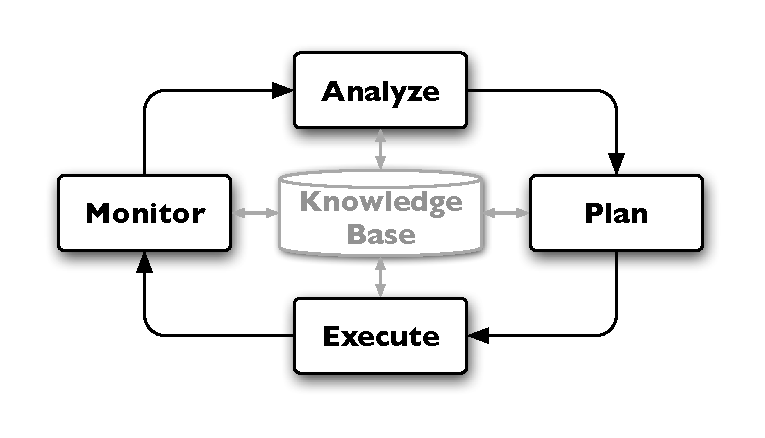
\includegraphics[width=0.5\textwidth]{mape.eps}
	\caption{General MAPE control loop}
	\label{fig:MAPE}
\end{figure}

Useful terminology is defined by \citet{IBM2006} in the field of autonomic computing. Figure \ref{fig:MAPE} shows an autonomic manager, which is a component that collects data from a system and, based on this data, performs actions with the purpose of improving the system. This control loop is divided into four subtasks called monitor (collect system information), analyze (correlate and model data), plan (design behavior required to reach goal) and execute (run the planned actions), sometimes referred to as MAPE. Each subtask can optionally interact with a knowledge base for storing and retrieving data. This will then be applied to online marketing.

\section{Marketing}
A number of marketing terms will be used throughout this paper. A \emph{marketing campaign}, or simply a \emph{campaign}, is comprised of one or more advertising messages, \emph{ads}, that are directed to one defined audience, the \emph{target} or \emph{target group}. Any ad, and by extension campaign, have numeric measures of success called \emph{metrics}. The most commonly used are \emph{impressions}, which is the number of times an ad has been shown, and clicks. In this paper however, the word \emph{action} will be used when referring to an user interaction, since one might be interested in other values than simple clicks, such as for example the number of users who go on to register at the site after clicking. Ads have a number of properties, which depend on the media that is used. For example, textual ads in search engines typically have a title, a short text and a URL to which the user is redirected upon clicking the ad. A target is defined based on the options available of the advertisement type used. A graphical description of these terms is shown in figure \ref{fig:MarketingTerminology}.

Four such classes are identified for the purpose of this paper based on the way the ads are adapted based on the user. \emph{Search} advertising uses the user's search terms, \emph{social} advertising uses demographic and personal data, \emph{contextual} advertising finds keywords on the page on which the ads are displayed or uses manual categorization and finally \emph{non-contextual} advertising, which does no relevancy matching. The separation between these classes is not necessarily distinct and a single publisher can use targeting criteria from different classes.

\begin{figure*}[htb] \centering 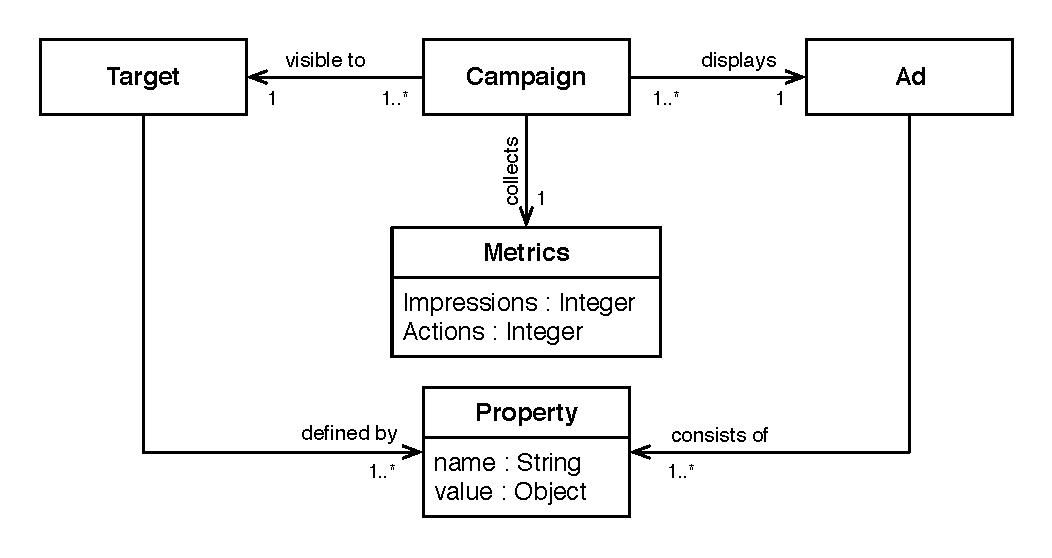
\includegraphics[width=0.9\textwidth]{marketing-uml.eps}
	\caption{UML description of marketing terminology.}
	\label{fig:MarketingTerminology}
\end{figure*}

As the word \emph{user} is typically used to refer to a person interacting with either the web site that is being marketed or the web site on which the advertisement is shown, we will use the word \emph{operator} when discussing a person interacting with the system that is described in this paper to avoid confusion.

\section{Automated marketing}
\begin{figure}[htb] \centering 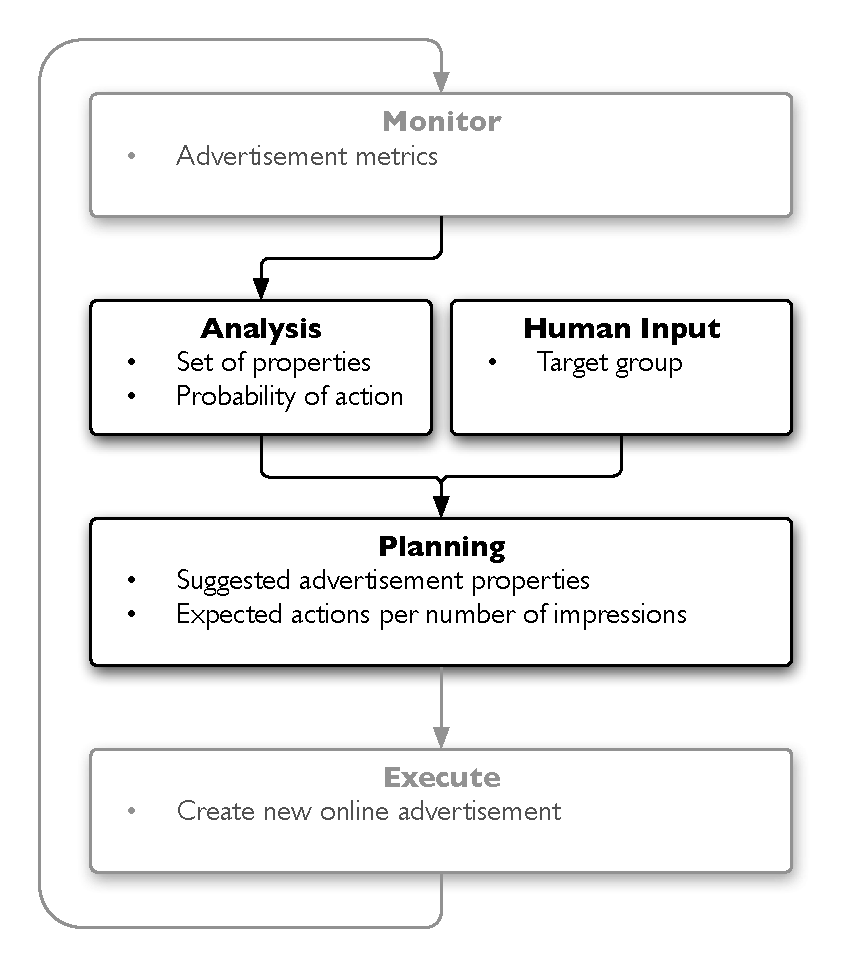
\includegraphics[width=0.5\textwidth]{mape-marketing.eps}
	\caption{Online marketing automation system in control loop}
	\label{fig:MAPEMarketing}
\end{figure}

By merging the fields of automation and online marketing we put the automation terminology in context. Monitoring is the collection of metrics for online advertisement. To optimize these metrics, the gathered information is analyzed and this analysis forms the basis for the planning of future campaigns. Once the plans are completed, the new campaign can be launched, with new metrics being gathered and so on.

Monitoring is commonly automated already, either using custom software or services such as Google Analytics, where as the other parts of the process are performed manually. It is infeasible to fully automate the whole process, due to for example the creative side of advertisement and the complex factors that decide which groups an upcoming campaign should target. There are however certain areas that can be automated and this paper will focus on automated analysis and planning of online marketing campaigns, shown in Figure \ref{fig:MAPEMarketing}.

A system to automate this process requires monitored data as input, which in this context equals historical data of campaigns and their metrics as mentioned previously. This data is then mined to identify subsets of campaign properties that are associated with a probability that an impression of that an ad with these properties leads to an action being taken by the user. Human input is required to specify which target group the next campaign will be aimed at, and based on this the system will generate suggested ad properties that optimize the number of expected actions taken per impression.

\section{Scope}
Using the MAPE framework in Figure \ref{fig:MAPE}, only the analysis and planning tasks are considered part of this paper, where as monitoring and execution are out of scope. The latter two are however relevant in the verification step, but will not be covered as a research topic. In this context, this means for example that the feature of integrating this system with marketing services to automatically add new ads and campaigns will not be a part of the final system.

Furthermore, the data set will likely include attributes whose values are free text and images. Text mining and image recognition are beyond the scope of this project. Instead these attributes will be manually categorized, so that the value space is discrete and finite.

\section{Foundations}
% Knowledge Discovery
A number of high-level descriptions of frameworks for knowledge discovery in databases exist \citep{Fayyad1996, Frawley1992} and they exhibit a number of commonalities. These include the importance of having a knowledgeable human operator guiding the process in terms of supplying domain knowledge to the system formulating the goal of the knowledge discovery; feeding discovered knowledge back into the system; and the identification and application of a discovery method, or more specifically the data mining algorithms.

% Data mining
In data mining, the input to a system can be described using the terms \emph{concepts}, \emph{instances} and \emph{attributes}, where concept is the actual result of the mining, i.e. what we want to be learned; an instance is one single example of data to be mined and can be compared to a row in a database; and attribute is a property of an instance, which in the database analogy is a column \citep{Witten2011}.

Instances are the smallest component of data input to a mining system, but its low-level description of knowledge may not be what is most useful. \citet{Chen1996} give an overview of the field of data mining where they mention the aspect of multi-level data mining, which states that correlations may not commonly exist on the lowest level of granularity, but instead by forming groups of related items. An example given would be that a specific brand of milk does not necessarily imply the purchase of a specific brand of bread, however purchasing milk of any kind may still be correlated to the purchase of bread irrespective of brand.

% Data mining algorithm classes, e.g. classifiers
% TODO: Write stuff

% Decision trees
In a highly influential paper, \citet{Quinlan1986} decribe how decision trees can be created from a training set and how well it handles the problem of unknown attributes values and noisy data. A related paper, \citet{Quinlan1987}, deal with how generated decision trees can be simplified in order to more easily be applied. Four different methods are evaluated, one of which is the reformulation of the tree as a set of production rules. This specific topic is further analyzed in \citet{Quinlan1987b} where such production rules are shown to be more compact and also in many cases improve the classification of unseen data. An added positive effect is that production rules from separate classifications can be merged more efficiently than their original decision trees.

% Case-based reasoning
% TODO: Belongs together with automation
Cased-based reasoning is a methodology that is similair in many ways to the automation framework described previously, but it is more closely related to human cognition. The basic concept as described in \citet{Watson1999} is that in order to solve a new problem, the first step is to identify (retrieve) existing problems that are similar. Select a solution to one of the retrieved problem and apply it to the current problem (reuse). Adapt (revise) the existing solution to better match the problem at hand, if necessary. Finally, store (retain) the problem and its solution if it was successful.

\chapter{Related works}
\citet{Richardson2007} describe a model for predicting the click-through rates of ads given a set of properties in the context of search engine advertisement. Though it is a relevant subject, the paper is limited to the specific class of search advertising, and is therefore not directly applicable to this paper.

In online advertisement there have been problems of so called click-spam or click-fraud, meaning that the number of clicks on ads is increased in a fraudulent manner, for example using bots. \citet{Dave2012} provides a methodology to measure click-spam in their networks as well as a study of the severity of the problem on different classes of networks. Their results show that established search advertising on for example Google and Bing is fairly accurate in their filtering of click-spam, where as the problem is  greater for contextual and social advertisement, and severe for mobile advertisement. A related paper by \citet{Zhang2011} describes a methodology for advertisers to evaluate the quality of click traffic and use this to assess the difference in quality between bulk traffic vendors and established pay-per-click networks.

Research has also shown that using targeted advertisement is effective given that the ad is not experienced as being obtrusive, though obstrusive ads that are not targeted also increase performance \citep{Goldfarb2011}. This promotes the idea of more effective targeting but may also be important to understand in how the solution presented in this thesis is applied.

Automation in marketing is not a completely novel idea. \citet{Joshi2006} present a technique for automatically finding related keywords for broader targeting of ads by creating a graph of search terms based on the domain knowledge contained in search engines. Continuation of that work is that of \citet{Thomaidou2011}, where keywords are also extracted from the landing page to further improve the results. Both approaches are however only relevant for contextual and search engine advertisement.

\chapter{Method}
The solution described in this paper is the result of thourough analysis of existing data sets as well as experiments. The method used to reach this solution is described in this chapter.

\chapter{Solution}
The solution has been divided into one section each for the two subtasks identified in the problem description. Analysis covers the problem of creating an appropriate model of the available data that is used in the next stage. Planning, in turn, is the utilization of that model with the purpose of outputting useful information to the operator. Finally, this is followed by the steps taken to evaluate the results.

\section{Analysis}
The first step in the process is analysis, and the first substep is how to deal with the input data. The data contains a set of metrics which are not best used in their raw form. The analysis step therefore calculates a confidence interval on the mean of the action rate, since it is more helpful in later processing steps than the more commonly used average action rate which do not take the size of the sample space into account.

The reason for specifying a confidence interval is to account for the inherit variance of values such as the action rate. Even though a campaign has been shown millions of times, there is still some degree of uncertainty to what the action rate would be if it was shown another million times. A \(100(1-\alpha)\%\) confidence interval is defined as the interval of values that a random variable \(X\) will take with a probability of \(1-\alpha\), or formally

\begin{equation}
	P[L_1 \leq X \leq L_2] = 1 - \alpha
\end{equation}

The standard function for calculating the values of the interval limits \(L_1\) and \(L_2\) is shown in equation \ref{eq:IntervalLimitsKnownVariance}.

\begin{equation}
	L = \bar{X} \pm z_{\alpha/2} \sigma/\sqrt{n}
	\label{eq:IntervalLimitsKnownVariance}
\end{equation}

The confidence interval is calculated based on the assumption of a normal distribution of the action rate. While the underlying distribution of each ad impression might not be normal, the Central Limit Theorem resolves that problem. The theorem defines that for a sample \(X_1, X_2, ..., X_n\) where \(n\) is large (empirically shown to work for \(n\) as low as 25), \(\bar{X}\) is approximately normal with mean \(\mu\) and variance \(\sigma^2/n\) \citep{Milton2002}.

At first look there is a problem with the use of a normal distribution. Because the variance is unknown and therefore needs to be estimated, this means that Student's t-distribution is more appropriate and that equation \ref{eq:IntervalLimitsUnknownVariance} should be used. However, because of the fact that \(t_{\alpha/2} \to z_{\alpha/2}\) as the degrees of freedom approaches infinity (at 2000 degrees of freedom, \(t_{0.025} \sim z_{0.025} \sim 1.96\) when rounded to two decimals), they are for all intents and purposes equal since we are typically working with impressions that quickly generate high degrees of freedom.

\begin{equation}
	L = \bar{X} \pm t_{\alpha/2} S/\sqrt{n}
	\label{eq:IntervalLimitsUnknownVariance}
\end{equation}

The distribution was also empirically tested using plotting to see that it follows the well-known bell curve of normal distributions as well as using the empirical rule, which states that for a normal distribution, about 68/95/99.7 percent of the values are respectively within 1/2/3 standard deviations of the mean.

After this processing, the data is added to the knowledge base for future use. The knowledge base will store all data relating to the marketing campaigns to increase the amount of available data to base decisions on.

Following this, additional data sets are created to support the planning phase. The idea is that ad properties are dealt with not only in combination but also as stand-alone entities to gain further insight into what makes ad work. Each ad property in every campaign instance from the data set is stored separately along with the campaign's metrics (i.e. impressions and actions). If an identical ad property value already exists, the metrics are aggregated so they reflect all occurrences of that property value.

\begin{figure}[htb] \centering 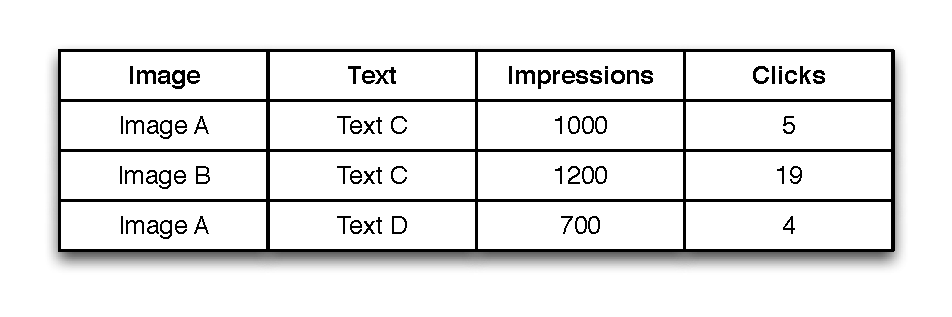
\includegraphics[width=0.8\textwidth]{data-set-example.eps}
	\caption{Data set example}
	\label{fig:DataSetExample}
\end{figure}

Figure \ref{fig:DataSetExample} shows an example of how the original data set could look like. The campaigns do not include any form of targeting and thus only consist of the ad properties image and text, as well as the metrics gathered, in this case impressions and clicks.

The second step of aggregating metrics for individual properties requires both impressions and clicks to be summed for each value of every ad property. For example, the data set for images would have one instance for Image A which has 1700 impressions and 9 clicks. The end result is shown in figure \ref{fig:DataSetPropertiesExample}.

\begin{figure}[htb] \centering 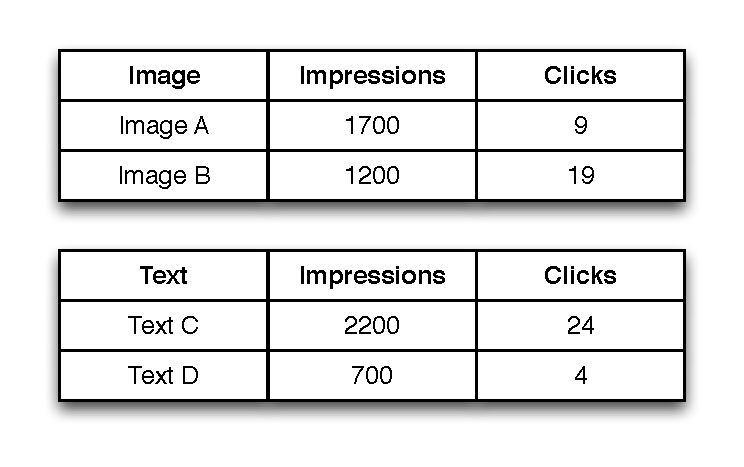
\includegraphics[width=0.6\textwidth]{data-set-properties-example.eps}
	\caption{Aggregating metrics in data set for each property value}
	\label{fig:DataSetPropertiesExample}
\end{figure}

For advertisers who also use targeting which is likely to impact the choice of ad properties, these additional data sets must be related to their respective targets and the aggregation of metrics should take this into account. For example, if the advertiser runs campaigns with images that target male and female users separetly, there will be one data set for images used on males and one data set for images used on females. An image used to target both sexes will thus appear in both of these data sets, but the metrics may be different.

\section{Planning}
The goal of the planning step is to formulate suggestions for upcoming campaigns. This is done by selecting values for each ad property that has an average action rate that lies above the mean of the property. Using the example in figure \ref{fig:DataSetPropertiesExample}, the mean is \((9+19)/(1700+1200) \approx .0097\) for images and \((24+4)/(2200+700) \approx .0097\) for texts, so Image B and Text C are selected for combination.

If the advertiser is running campaigns with different target groups, the basis for the planning must only be properties that are used with the specific target groups decided upon by the operator.

For every combination, an estimate of the real action rate is created. In the case of the above example, there is already an existing campaign in the knowledge base that is identical, so the actual action rate of that ad (or the average of all identical campaigns, if there are more than one) is used as an estimate.

An interesting and likely problem arises when the combination has never been used before. Once again using the example data set, the combination Image B and Text D does not exist previously so a method for estimating the action rate for such campaigns must be defined.

Existing variables to base the estimate on are the metrics for each property, but they are not enough by themselves since one property may carry a stronger influence on the actual result than another. The Pearson coefficient of correlation is such a measure and it is defined as

\begin{equation}
	\rho = \frac{Cov(X, Y)}{\sqrt{(Var X)(Var Y)}}
\end{equation}

Because the covariance and variance are unknown they have to be estimated based on the sample.

\begin{equation}
	\hat{\rho} = \frac{\widehat{Cov(X, Y)}}{\sqrt{(\widehat{Var X})(\widehat{Var Y})}} = \frac{ \sum_{i=1}^{n} (X_i - \bar{X})(Y_i - \bar{Y}) }{ \sqrt{ (\sum_{i=1}^{n} (X_i - \bar{X})^2) (\sum_{i=1}^{n} (Y_i - \bar{Y})^2) } }
\end{equation}

Because \(-1 \leq \hat{\rho} \leq 1 \), where a value of 1 or -1 means there is an exact linear correlation between the two random variables and 0 means there is no linear correlation at all, values for the correlation of \(X_1\) and \(X_2\)in relation \(Y_0\) are comparable. This is useful to get an understanding of which variable most strongly influences the value of the dependent variable and also whether that influence is positive or negative.

Another possible solution to identifying the correlation is to use multiple linear regression. The general linear model is defined as

\begin{equation}
	\mu_{Y|x_1,x_2,\dotsc,x_k} = \beta_0 + \beta_1 x_1 + \beta_2 x_2 + \dotsc + \beta_k x_k
\end{equation}

where \(\mu\) is the mean of \(Y\) given values for its dependent variables \citep{Milton2002}. The \(\beta\)-values define the change in \(\mu\) for each unit of change in the related \(x\), and could as such be used as some form of correlation measure. This approach would be useful if the linear regression model could provide good estimates for the dependent variable's value, but empirical analysis on this project showed a much too great variance for the model to be useful for this purpose. As such, using linear regression cannot provide any additional value than the simpler Pearson coeffiecient.

The variables available for basing the estimation for the combination of two different properties X and Y are thus the low and high values of the action rate confidence interval, refered to as \(x_{low}\), \(x_{high}\), \(y_{low}\) and \(y_{high}\) respectively, as well as the correlation coefficient for each attribute, \(\rho_x\) and \(\rho_y\). The idea behind the estimation function is to sum the average action rate of each property, which is weighted depending on how much the property tends to influence the result, and normalize that sum. Using the previously mentioned variables, the estimation function is described as the following inequality.

\begin{equation}
	\frac{\rho_x x_{low} + \rho_y y_{low}}{\rho_x + \rho_y} \leq z \leq \frac{\rho_x x_{high} + \rho_y y_{high}}{\rho_x + \rho_y}
\end{equation}

Finally, the estimates are used to rank suggested campaigns based on the likelihood of resulting in high action rates. This is to provide decision support for domain experts who handle the final execution of marketing campaigns.

\section{Rate estimation}
To validate the regression model as a sufficient mean of estimation, we used an actual data set from Duego. The data set was randomly split into two separate, non-overlapping sets called training and validation. The training set was then used to create the regression model, after which the action rate of the validation instances was estimated. For each such estimate, an estimate was considered successful if the following inequality held.

\[
	c_i - \epsilon \leq \hat{c}_i \leq c_i + \epsilon
\]

\(c_i\) is the actual action rate from the validation set and \(\hat{c}_i\) the estimated value. The tolerance limit is defined as \(\epsilon = k*\bar{c}\), where \(k\) is a constant between 0 and 1. This process was repeated 5000 times and both the total number of estimations as well as the number of successful estimations were counted. From this a success percentage was calculated for different values of \(k\). Table \ref{tbl:EstimationSuccess} and Figure \ref{fig:EstimationSuccess} show the results of this experiment.

\begin{table}[htbp]
\begin{center}
	\begin{tabular}{  l | r r r r }
		\hline
		\textbf{Method} & \textbf{k=0.01} & \textbf{k=0.05} & \textbf{k=0.10} & \textbf{k=0.20} \\
		\hline
		Uniform distribution (range) & 1.51\% & 7.41\% & 14.32\% & 29.74\% \\
		Normal distribution & 2.55\% & 12.99\% & 25.72\% & 48.50\% \\
		Regression model & 1.90\% & 14.78\% & 33.40\% & 72.64\% \\
		\hline
	\end{tabular}
	\caption{Estimation success percentage over 5000 rounds}
	\label{tbl:EstimationSuccess}
\end{center}
\end{table}

\begin{figure}[htbp]
\begin{center}
	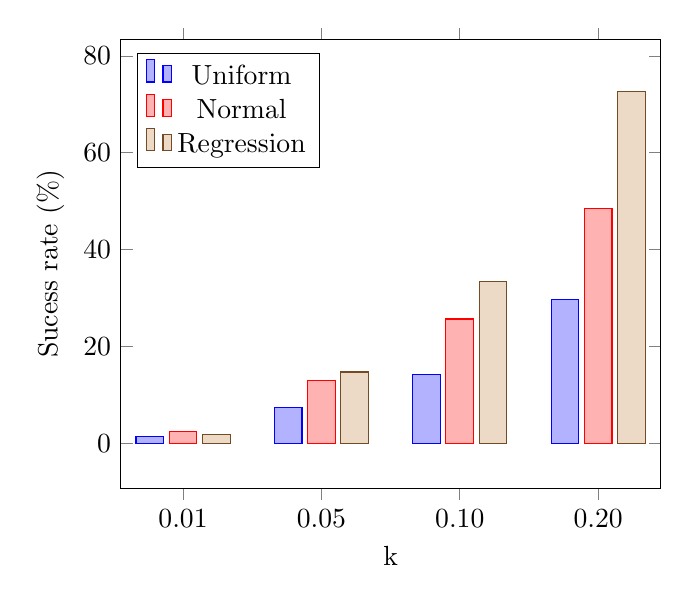
\begin{tikzpicture} \begin{axis}[
	    ybar,
	    enlargelimits=0.15,
	    legend pos=north west,
	    ylabel={Sucess rate (\%)},
	    xlabel={k},
	    symbolic x coords={0.01,0.05,0.10,0.20},
	    xtick=data,
	    ]
	\addplot coordinates {(0.01, 1.505) (0.05, 7.405) (0.10, 14.315) (0.20, 29.74)};
	\addplot coordinates {(0.01, 2.55) (0.05, 12.99) (0.10, 25.72) (0.20, 48.50)};
	\addplot coordinates {(0.01, 1.895) (0.05, 14.775) (0.10, 33.395) (0.20, 72.635)};
	\legend{Uniform,Normal,Regression}
	\end{axis}
	\end{tikzpicture}
	\caption{Bar chart of Table \ref{tbl:EstimationSuccess}}
	\label{fig:EstimationSuccess}
\end{center}
\end{figure}

As \(k\) increases it becomes clear that the regression model is noticibly better than the statistical distributions. Additional experiments revealed that the regression model reached a 50\% success rate at \(k \approx 0.135\).

\section{Selection strategy}
Once the estimations are made the question becomes how to select which ads to run. Obviously it is reasonable to assume that higher estimates are more likely to perform well, but it is less obvious whether a higher action rate can be expected by selecting multiple ads from the estimates.

Strategy N is defined as the selection strategy where the N highest estimated ads are selected and run. In addition to this, the ads can be run either weighted or unweighted. The latter means that all ads are shown the same amount of times, where as the former approach calculates a weight for each ad based on the normalized value of the estimate. The average real action rate is calculated as shown below. This process was then repeated 5000 times and the values averaged to identify the optimal selection strategy. The results are available in Table \ref{tbl:SelectionStrategy}.

\[
	c_{unweighted} = \sum_{i=1}^{N} \frac{ c_i }{ N }
\]
\[
	c_{weighted} = \frac{ \sum_{i=1}^{N} \hat{c}_i \cdot c_i }{ \sum_{i=1}^{N} \hat{c}_i }
\]

\begin{table}
\begin{center}
	\begin{tabular}{  l | r  r  }
		\hline
		\textbf{No. of ads} & \textbf{Unweighted} & \textbf{Weighted} \\
		\hline
		1 & 0.0214\% & 0.0214\% \\
		2 & 0.0209\% & 0.0209\% \\
		3 & 0.0206\% & 0.0206\% \\
		\hline
	\end{tabular}
	\caption{Averaged real action rate for selection strategies}
	\label{tbl:SelectionStrategy}
\end{center}
\end{table}

\section{Evaluation}
For the system to be useful to the advertiser, the final estimates for suggested campaigns must be accurate enough so they can be trusted by the domain experts making decisions on which campaigns to run. As the combining of possibly unrelated ad properties may give rise to more uncertainty than what existed when those same properties were considered separatly, the estimation function needs to be evaluated.

The system is tested by using using the available infrastructure for managing marketing campaigns at Duego. The test consists of selecting ten suggested campaigns to run live. After each campaign has gathered at least half a million impressions, the final mean action rate is calculated and compared to the original estimate. If a 90\% confidence interval on the action rates used as the basis for estimation is chosen, and assuming this confidence interval is applicable to the estimates as well, there is a 10\% chance that the mean action rate from the test is not in the interval. The results are considered to be validated if no more than two of the ten campaigns fall outside of the estimated intervals.

\chapter{Discussion}
\section{Risk factors}
Because the output of the system is dependent on historical data, an assumption has been made that older data is still representative of the current state of the marketing. This is definitely not true for campaigns that are adapted for Christmas, Valentine's Day or other special occasions. The assumption is that the amount of such time-dependent data is so small that it will not impact the final results. If however there is reason to believe that this set of data would influence the output, the recommended approach is to remove it from the knowledge base.

\section{Future work}
This paper uses a very simple similarity measure for the targeting because it is not a central part of the thesis. For advertisers with many campaigns with differing targeting it would probably be interesting to develop a more advanced form of measure. Certain attributes may not have a binary relation (related or not related) but rather they may themselves have a similarity score. An example of this could be age, where the similarity score in this paper would be zero for two targets of age 19 and 20 respectively, though in reality it seems likely that these groups would be attracted to the same properties in an ad.

\chapter{Conclusion}
Empty.

\bibliography{references} % references.bib
\addcontentsline{toc}{chapter}{\numberline{} Bibliography} % For pdf
\setspecialhdr

\newpage

% Appendices
\appendix
\setdefaulthdr
%\input{include/appendix1}
\end{document}